% ============================================================================
% Directional Curvature Expansion of the Baker Cubic Coefficient on Riemannian
% Surfaces Through Fifth Order -- Version 2.5 (October 29, 2026)
% Revision of v2.3 (September 29, 2026).
%
% RELEASE REVIEW NOTES:
%  * Reported external transcription test requires the actual script for local verification.
%  * No equation, coefficient, table value or numerical result of v2.3 was changed.
%  * New in v2.4: Section 9 (independent verification), provenance/disclosure,
%    wording of the rigor claim, uniformity/parity clarifications, scope remark.
%  * Companion script curvature_v24_checks.py reproduces Section 9 (26 checks).
% ============================================================================
\documentclass[11pt]{amsart}

\usepackage[T1]{fontenc}
\usepackage[utf8]{inputenc}
\usepackage{lmodern}
\usepackage{amsmath,amssymb,amsthm,mathtools}
\usepackage{booktabs}
\usepackage{graphicx}
\usepackage{xcolor}
\usepackage{microtype}
\usepackage{enumitem}
\usepackage{tikz}
\usetikzlibrary{arrows.meta,calc}
\usepackage{pgfplots}
\pgfplotsset{compat=1.18}
\usepackage{placeins}
\usepackage[colorlinks=true,linkcolor=blue,citecolor=blue,urlcolor=blue,pdftitle={Directional Curvature Expansion of the Baker Cubic Coefficient on Riemannian Surfaces Through Fifth Order},pdfauthor={Wayne Baker},pdfkeywords={Riemannian normal coordinates, geodesic distance, Gaussian curvature, local invariants}]{hyperref}
\usepackage[capitalise,nameinlink,noabbrev]{cleveref}
\usepackage[margin=1in]{geometry}

\numberwithin{equation}{section}

\newtheorem{theorem}{Theorem}[section]
\newtheorem{proposition}[theorem]{Proposition}
\newtheorem{lemma}[theorem]{Lemma}
\newtheorem{corollary}[theorem]{Corollary}
\theoremstyle{remark}
\newtheorem{remark}[theorem]{Remark}

\newcommand{\Riem}{\mathcal{R}}
\newcommand{\BRiem}{\widetilde{R}}
\newcommand{\Cthree}{C_3}
\newcommand{\bigO}{\mathcal{O}}
\newcommand{\Hess}{\nabla^2}
\newcommand{\Third}{\nabla^3}
\newcommand{\dd}{\mathrm{d}}
\newcommand{\Span}{\operatorname{span}}

\newif\ifflags
\flagstrue
\newcommand{\flag}[1]{\ifflags{\textbf{\color{red}[VERIFY: #1]}}\fi}

\title[Directional curvature expansion]{Directional Curvature Expansion of the Baker Cubic Coefficient on Riemannian Surfaces Through Fifth Order}
\author{Wayne Baker}
\address{Independent researcher}
\date{Version 2.5 --- October 29, 2026\\ First version: September 29, 2026}

\subjclass[2020]{53B20, 53A55, 65D30}
\keywords{Riemannian normal coordinates, geodesic distance, local invariants, Gaussian curvature, asymptotic expansion, geometric refinement}

\begin{document}

\begin{abstract}
Let $p$ be a point of a smooth Riemannian surface, let $w\in T_pM$ be a unit bisector direction, and let $\rho$ be the radius of a sufficiently small geodesic circle.  A symmetric pair of radial geodesics determines an intrinsic signed side-length law.  Encoding an angular error by this side length, multiplying by a scale $q>1$, and decoding through the inverse side law produces an odd local defect map whose leading term is cubic.  We derive the complete directional curvature expansion of its cubic coefficient through order $\rho^5$.  For the scale $q=4/3$ arising in the Baker approximate-trisection refinement, the result is
\[
\begin{aligned}
C_3(p,w,\rho)
={}&-\frac7{384}+\frac7{384}K\rho^2
+\frac7{512}(\nabla_wK)\rho^3\\
&+\left[-\frac7{1152}K^2-\frac7{7680}\Delta K
+\frac{49}{7680}\nabla^2K(w,w)\right]\rho^4\\
&+\left[-\frac{21}{2560}K\nabla_wK
-\frac7{11520}\nabla_w\Delta K
+\frac{49}{23040}\nabla^3K(w,w,w)\right]\rho^5
+\bigO(\rho^6).
\end{aligned}
\]
The proof combines Brewin's corrected degree-six and degree-seven two-point distance expansions with exact surface tensor reduction and a short encode--scale--decode inversion.  Orientation reversal removes all mixed components with an odd number of $Jw$ slots, while direction reversal forces the alternating even--odd invariant structure.  The coefficients are checked symbolically with exact rational arithmetic, against the exact spherical law and the classical small-circle expansion, and by independent high-precision intrinsic-geodesic computations on a ring torus.  Symmetric averages independently recover the quartic coefficient, while four meridional latitudes---including a negative-curvature point---give an overdetermined fifth-order invariant system and numerically recover all three weight-five multipliers.  The result is derived from Brewin's published degree-six and degree-seven formulas, which are used as source data and not rederived; Section~\ref{sec:verify} records independent re-implementations of their surface reduction, a transcription comparison, and an endpoint-swap symmetry test. The normal-coordinate and invariant-theoretic machinery is classical; the contribution is the explicit realization and exact coefficient determination for this intrinsic cubic refinement law.
\end{abstract}

\maketitle

\section{Introduction}

Approximate geometric constructions often admit local error maps whose leading nonlinear coefficient is universal in Euclidean geometry but acquires curvature corrections on a Riemannian surface.  The construction considered here originates in a straightedge-and-compass approximate angle-trisection method due to the author and documented by Rostamian~\cite{Rostamian}.  Its Euclidean refinement law has a cubic leading defect.  The purpose of this paper is not to revisit exact angle trisection, but to study the intrinsic local coefficient produced when the same encode--scale--decode mechanism is placed on a smooth surface.

The central object is a signed side-length law on a small geodesic circle.  Two equal-radius radial directions are placed symmetrically about a unit vector $w$, with signed angular separation $x$.  Their endpoints have intrinsic distance $c_{\rho,w}(x)$.  The map $x\mapsto c_{\rho,w}(x)$ is locally odd and invertible.  The encoded side length is multiplied by a fixed scale $q>1$, decoded through the inverse side law, and compared with the original angular error.  Oddness forces the calibrated defect map to contain only odd powers of the error variable, so the first nonlinear coefficient is cubic.

The Euclidean coefficient is $-7/384$ at the scale $q=4/3$.  On a sphere of constant positive curvature, the exact coefficient is $-(7/384)\cos^2(\sqrt K\,\rho)$.  These facts suggest a local curvature expansion, but they do not determine the directional terms on variable-curvature surfaces.  The terms through $\rho^3$ follow from the classical degree-five two-point distance expansion.  The present work derives the degree-six and degree-seven contributions and thereby determines the coefficient through $\rho^5$.

The coefficient is mathematically useful beyond its origin in approximate trisection because a single scalar observable separates successive layers of local surface geometry.  The $\rho^2$ and $\rho^3$ terms recover $K$ and its directional derivative, while the next two orders resolve the even weight-four basis $\{K^2,\Delta K,\nabla^2K(w,w)\}$ and the odd weight-five basis $\{K\nabla_wK,\nabla_w\Delta K,\nabla^3K(w,w,w)\}$.  Thus the trisection construction supplies the motivating refinement law, while the Riemannian problem is to determine exactly how that intrinsic law organizes local curvature invariants.

The required two-point geodesic-distance coefficients come from the corrected v3 version of Brewin's normal-coordinate calculation~\cite{Brewin2009}.  Brewin's public Cadabra and LaTeX repository provides an implementation-level source for the same formulas~\cite{BrewinRepository}.  Because higher-order normal-coordinate formulas are convention-sensitive, we first verify that Brewin's lower-order terms reproduce the curvature convention used here.  Only then are the degree-six and degree-seven formulas reduced on a surface.

The resulting invariant pattern alternates with the radial order:
\[
\begin{array}{c|c|l}
\text{order} & w\mapsto-w & \text{invariants}\\
\hline
\rho^2 & \text{even} & K,\\
\rho^3 & \text{odd} & \nabla_wK,\\
\rho^4 & \text{even} & K^2,\ \Delta K,\ \nabla^2K(w,w),\\
\rho^5 & \text{odd} & K\nabla_wK,\ \nabla_w\Delta K,\ \nabla^3K(w,w,w).
\end{array}
\]
This is consistent with classical local invariant theory~\cite{Gilkey,GrahamKuo2026}.  We do not claim the invariant-weight framework itself as new.  The new content is the reduction of the intrinsic encode--scale--decode law to this invariant basis and the exact determination of all coefficient multipliers through radial order five, together with source-locked symbolic and independent numerical checks.

\subsection*{Main result}
All curvature quantities below are evaluated at $p$.

\begin{theorem}[General scale and Baker specialization]\label{thm:main}
Let $(M,g)$ be a smooth Riemannian surface, $p\in M$, $w\in T_pM$ a unit vector, and let $\rho>0$ be sufficiently small that the geodesic circle of radius $\rho$ lies in a convex normal neighbourhood of $p$.  For $q>1$, let $C_{3,q}(p,w,\rho)$ be the calibrated cubic coefficient defined in \cref{sec:definition}.  Then
\begin{align}
C_{3,q}(p,w,\rho)
={}&\frac{q^2-1}{q^2}\Bigg[
-\frac1{24}+\frac1{24}K\rho^2+\frac1{32}(\nabla_wK)\rho^3 \notag\\
&+\left(-\frac1{72}K^2-\frac1{480}\Delta K
+\frac7{480}\Hess K(w,w)\right)\rho^4 \notag\\
&+\left(-\frac3{160}K\nabla_wK
-\frac1{720}\nabla_w\Delta K
+\frac7{1440}\Third K(w,w,w)\right)\rho^5
+\bigO(\rho^6)\Bigg].
\label{eq:general-main}
\end{align}
For the Baker scale $q=4/3$, write $C_3=C_{3,4/3}$.  Then
\begin{align}
C_3(p,w,\rho)
={}&-\frac7{384}+\frac7{384}K\rho^2
+\frac7{512}(\nabla_wK)\rho^3 \notag\\
&+\left[-\frac7{1152}K^2-\frac7{7680}\Delta K
+\frac{49}{7680}\Hess K(w,w)\right]\rho^4 \notag\\
&+\left[-\frac{21}{2560}K\nabla_wK
-\frac7{11520}\nabla_w\Delta K
+\frac{49}{23040}\Third K(w,w,w)\right]\rho^5
+\bigO(\rho^6).
\label{eq:baker-main}
\end{align}
\end{theorem}

The proof occupies \cref{sec:definition,sec:distance,sec:surface,sec:side}.  Exact checks and independent numerical validation are presented in \cref{sec:checks,sec:numerics}.  The theorem is proved \emph{relative to} Brewin's published degree-six and degree-seven two-point distance formulas (Appendix~\ref{app:source}), which are taken as input and are not rederived here; independent checks of their transcription and surface reduction are recorded in \cref{sec:verify}.

\section{Intrinsic side law and cubic defect coefficient}\label{sec:definition}

Fix a local orientation at $p$ and let $J:T_pM\to T_pM$ be rotation through $\pi/2$.  For a small signed angular separation $x$, put
\begin{equation}\label{eq:directions}
 u_x=\cos\frac{x}{2}\,w-\sin\frac{x}{2}\,Jw,
 \qquad
 v_x=\cos\frac{x}{2}\,w+\sin\frac{x}{2}\,Jw.
\end{equation}
The vectors $u_x$ and $v_x$ are symmetric about $w$ and have signed angular separation $x$.  For $x\ge0$, define
\[
 \widehat c_{\rho,w}(x)
 =d\!\left(\exp_p(\rho u_x),\exp_p(\rho v_x)\right),
\]
and define its odd extension by
\begin{equation}\label{eq:signed-side}
 c_{\rho,w}(x)=
 \begin{cases}
 \widehat c_{\rho,w}(x),&x>0,\\
 0,&x=0,\\
 -\widehat c_{\rho,w}(-x),&x<0.
 \end{cases}
\end{equation}
For sufficiently small $x$, this is a smooth odd local coordinate with positive derivative at the origin.

\begin{figure}[htbp]
\centering
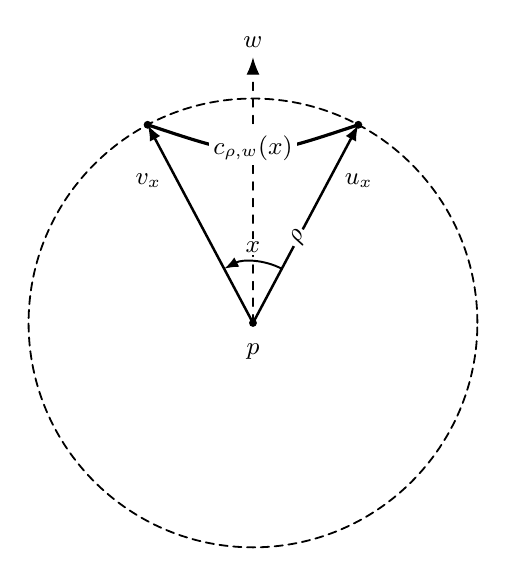
\begin{tikzpicture}[scale=0.95,line cap=round,line join=round,>=Latex,every node/.style={font=\small}]
  \coordinate (p) at (0,0);
  \coordinate (U) at (62:3);
  \coordinate (V) at (118:3);
  \draw[densely dashed,line width=0.65pt] (p) circle[radius=3];
  \draw[dashed,-{Latex[length=2.2mm]}] (p)--(0,3.55) node[above] {$w$};
  \draw[line width=0.9pt,-{Latex[length=2mm]}] (p)--(U) node[pos=0.72,right=2pt] {$u_x$};
  \draw[line width=0.9pt,-{Latex[length=2mm]}] (p)--(V) node[pos=0.72,left=2pt] {$v_x$};
  \fill (p) circle[radius=1.5pt] node[below=4pt] {$p$};
  \fill (U) circle[radius=1.5pt];
  \fill (V) circle[radius=1.5pt];
  \node[rotate=62,fill=white,inner sep=1pt] at ($(p)!0.43!(U)$) {$\rho$};
  \draw[-{Latex[length=1.8mm]},line width=0.7pt] (62:0.82) arc[start angle=62,end angle=118,radius=0.82];
  \node[fill=white,inner sep=1pt] at (0,1.02) {$x$};
  \draw[line width=1.15pt] (U)..controls(0,2.18)..(V);
  \node[fill=white,inner sep=1.5pt] at (0,2.34) {$c_{\rho,w}(x)$};
\end{tikzpicture}
\caption{Symmetric equal-radius endpoint geometry.  The drawing is schematic; all distances in the definition are intrinsic.}
\label{fig:geometry}
\end{figure}

For a scale factor $q>1$, define the local encode--scale--decode map $\Phi_{\rho,w,q}$ by
\begin{equation}\label{eq:phi}
 c_{\rho,w}(\Phi_{\rho,w,q}(x))=q\,c_{\rho,w}(x),
 \qquad \Phi_{\rho,w,q}(0)=0,
\end{equation}
using the branch with positive derivative.  The calibrated defect map is
\begin{equation}\label{eq:defect}
 F_{\rho,w,q}(e)=e-\Phi_{\rho,w,q}(e/q).
\end{equation}
Oddness of the side law and its inverse implies
\begin{equation}\label{eq:error-spectrum}
 F_{\rho,w,q}(e)=C_{3,q}(p,w,\rho)e^3+C_{5,q}(p,w,\rho)e^5+\cdots.
\end{equation}
Thus even powers of the error variable are structurally forbidden before any extrapolation is applied.

\begin{lemma}[Coefficient ratio]\label{lem:ratio}
If
\[
 c_{\rho,w}(x)=b_1(\rho)x+b_3(\rho)x^3+\bigO(x^5),
\]
then
\begin{equation}\label{eq:ratio-identity}
 C_{3,q}(p,w,\rho)=\frac{q^2-1}{q^2}\frac{b_3(\rho)}{b_1(\rho)}.
\end{equation}
\end{lemma}

\begin{proof}
Write $\Phi(x)=qx+Ax^3+\bigO(x^5)$.  Comparing cubic coefficients in $c(\Phi(x))=q c(x)$ gives
\[
 b_1A+b_3q^3=qb_3,
 \qquad
 A=q(1-q^2)\frac{b_3}{b_1}.
\]
Substitution into $F(e)=e-\Phi(e/q)$ yields \eqref{eq:ratio-identity}.  In particular, no $x^5$ coefficient of the side law is required to determine the cubic defect coefficient.
\end{proof}

\section{Two-point distance expansion and convention lock}\label{sec:distance}

We use
\[
 R(A,B)C=\nabla_A\nabla_BC-\nabla_B\nabla_AC-\nabla_{[A,B]}C,
 \qquad
 \Riem(A,B,C,D)=\langle R(A,B)C,D\rangle,
\]
so that on a surface
\begin{equation}\label{eq:R-convention}
 \Riem(A,B,B,A)=K\bigl(|A|^2|B|^2-\langle A,B\rangle^2\bigr).
\end{equation}
Positive Gaussian curvature therefore gives a positive value in the slots $(A,B,B,A)$.

In component notation, the geometric four-slot tensor therefore satisfies
\begin{equation}\label{eq:R-components}
 \Riem_{abcd}
 =K\left(g_{ad}g_{bc}-g_{ac}g_{bd}\right).
\end{equation}
Brewin's displayed arc-length formulas use a component array with the
opposite four-slot sign relative to this convention.  We therefore define
\begin{equation}\label{eq:brewin-array}
 \BRiem_{abcd}
 :=-\Riem_{abcd}
 =K\left(g_{ac}g_{bd}-g_{ad}g_{bc}\right).
\end{equation}
All transcriptions of Brewin's Equations 11.21b--e below use the source
array $\BRiem$.  This distinction is essential because the geometric tensor
and Brewin's component array have opposite signs in the relevant slot
ordering.

The lower-order two-point expansion may be written
\begin{align}
 d(\exp_pX,\exp_pY)^2
={}&|X-Y|^2-\frac13\Riem(X,Y,Y,X)\notag\\
&-\frac1{12}(\nabla_{X+Y}\Riem)(X,Y,Y,X)
+\bigO((|X|+|Y|)^6).
\label{eq:lower-distance}
\end{align}
This agrees with the distance expansion used by Pennec after conversion to the convention \eqref{eq:R-convention}~\cite[Eq.~(9)]{Pennec2019}.  For the higher orders we use Brewin's corrected v3 arc-length formulas~\cite{Brewin2009}.  The arXiv record notes that v2 corrected computational errors and v3 corrected an index/sign issue in a separate group of displayed formulas; the repository contains the revised Cadabra and LaTeX sources~\cite{BrewinRepository}.

Write the squared-distance expansion in the form
\begin{equation}\label{eq:Hn-definition}
d(\exp_pX,\exp_pY)^2=|D|^2+\sum_{n\ge4}H_n(X,D),
\end{equation}
where $H_n$ denotes the homogeneous degree-$n$ contribution in $(X,D)$ in Brewin's normal-coordinate expansion.

  The remainder after the displayed homogeneous terms admits the following local factorization.

\begin{lemma}[Uniform normalized remainder]\label{lem:uniform-remainder}
Fix a point $p$ and a sufficiently small convex normal neighbourhood. Let
$D=Y-X$, and write $d^2(\exp_pX,\exp_pY)=|D|^2+E(X,D)$.
After subtracting the homogeneous terms of total degree at most seven, the
remainder along \eqref{eq:XD} can be written
\[
 E_{\geq8}(\rho,x)=4\rho^2s(x)^2\,\rho^6\mathcal R(\rho,x,w),
\]
where $\mathcal R$ is jointly smooth near $(\rho,x)=(0,0)$, uniformly in unit
directions $w$. In particular its $x$ derivatives of each fixed finite order
are bounded locally, so normalized coefficient extraction through radial
order five carries a uniform $O(\rho^6)$ remainder. The normalized squared
side law is even in $x$ under endpoint interchange.
\end{lemma}
\begin{proof}
In the smooth coordinates $(X,D)$, the function $E$ vanishes at $D=0$
together with its first derivative in $D$. Indeed the squared distance and
$|D|^2$ both have a zero of order at least two on the diagonal. The iterated
integral form of Hadamard's lemma yields
\[
 E(X,D)=D^aD^bF_{ab}(X,D),\qquad
 F_{ab}(X,D)=\int_0^1(1-t)\,\partial_{D^a}\partial_{D^b}E(X,tD)\,dt,
\]
with $F_{ab}$ smooth. Taylor expansion of $F_{ab}$ in the joint variables
$(X,D)$ through total degree five has an integral remainder of order six,
whose coefficient is smooth jointly in the expansion parameters. Multiplying
by $D^aD^b$ gives exactly the omitted total-degree-eight-and-higher terms.
Along \eqref{eq:XD}, $X,D$ are smooth and $O(\rho)$ and
$D=2\rho s(x)Jw$. Hence the Taylor remainder is
$4\rho^2s(x)^2\rho^6\mathcal R(\rho,x,w)$, with smooth $\mathcal R$.
Compactness of the unit tangent circle supplies uniform local bounds in $w$.
The interchange of the two endpoints sends $x$ to $-x$, leaving their
squared distance unchanged; the factor $4\rho^2s(x)^2$ is also even. Thus
the normalized squared side law is even in $x$. The locally positive
normalized square root is smooth, and differentiating its $x$-Taylor
coefficients preserves the claimed radial remainder. Since
$b_1(\rho)/\rho\to1$, division to form $b_3/b_1$ also preserves it.
\end{proof}

Brewin writes $x=X$ and $Dx=D=Y-X$.  His Equations 11.21b--c are
\begin{equation}\label{eq:brewin-b}
 3H_4=-X^aX^bD^cD^d\BRiem_{acbd},
\end{equation}
\begin{equation}\label{eq:brewin-c}
 12H_5=-X^aX^bD^cD^dD^e\nabla_c\BRiem_{adbe}
 -2X^aX^bX^cD^dD^e\nabla_a\BRiem_{bdce}.
\end{equation}

\begin{lemma}[Generic convention checksum]\label{lem:checksum}
Under \eqref{eq:R-convention}--\eqref{eq:brewin-array}, \eqref{eq:brewin-b}--\eqref{eq:brewin-c} reproduce exactly the two curvature terms in \eqref{eq:lower-distance}.
\end{lemma}

\begin{proof}
Define $\Omega(U,V)^2=|U|^2|V|^2-\langle U,V\rangle^2$.  Because $D=Y-X$, one has $\Omega(X,D)=\Omega(X,Y)$.  On a surface,
\[
 X^aX^bD^cD^d\BRiem_{acbd}=K\Omega(X,D)^2=\Riem(X,Y,Y,X),
\]
which proves the $H_4$ identity.  Since $\nabla g=0$,
\[
 \nabla_m\BRiem_{abcd}=(\nabla_mK)(g_{ac}g_{bd}-g_{ad}g_{bc}).
\]
The two contractions in \eqref{eq:brewin-c} reduce to
\[
 (\nabla_DK)\Omega(X,D)^2,
 \qquad
 (\nabla_XK)\Omega(X,D)^2.
\]
Their weighted sum is $(\nabla_DK+2\nabla_XK)\Omega(X,D)^2=(\nabla_{X+Y}K)\Omega(X,Y)^2$ because $D+2X=X+Y$.  This gives the $H_5$ identity.
\end{proof}

This lower-order checksum is performed symbolically for generic vectors before either higher-order formula is used.

\section{Surface reduction through homogeneous degree seven}\label{sec:surface}

Put
\[
 s=\sin\frac{x}{2},\qquad c=\cos\frac{x}{2},
 \qquad X=\rho(cw-sJw),\qquad Y=\rho(cw+sJw),
\]
so that
\begin{equation}\label{eq:XD}
 D=Y-X=2\rho sJw,
 \qquad X+Y=2\rho cw,
 \qquad |X-Y|^2=4\rho^2s^2.
\end{equation}
Let
\[
 G_{abcd}=g_{ac}g_{bd}-g_{ad}g_{bc}.
\]
The Brewin source array satisfies $\BRiem=KG$, and $G$ is parallel.  Hence
\begin{equation}\label{eq:derivative-reduction}
 \nabla\BRiem=(\nabla K)\otimes G,
 \qquad
 \nabla^2\BRiem=(\nabla^2K)\otimes G,
 \qquad
 \nabla^3\BRiem=(\nabla^3K)\otimes G,
\end{equation}
with derivative ordering inherited from Brewin's formula.

\subsection{Orders \texorpdfstring{$\rho^2$ and $\rho^3$}{rho2 and rho3}}
From \eqref{eq:lower-distance},
\begin{equation}\label{eq:A2A3}
 c_{\rho,w}(x)^2
 =4\rho^2s^2\left[1+A_2\rho^2+A_3\rho^3+\bigO(\rho^4)\right],
\end{equation}
where
\begin{equation}\label{eq:A2A3-values}
 A_2=-\frac13Kc^2,
 \qquad
 A_3=-\frac16(\nabla_wK)c^3.
\end{equation}
The first term is isotropic; the first directional term is odd under $w\mapsto-w$.

\subsection{Homogeneous degree six}
Choose the orthonormal frame $e_1=w$, $e_2=Jw$ and write
\[
 H_{11}=\Hess K(w,w),\quad H_{12}=\Hess K(w,Jw),\quad H_{22}=\Hess K(Jw,Jw).
\]
Brewin's Equation 11.21d contains three polynomial blocks.  Exact contraction of those blocks gives
\begin{align*}
T_{1,R}&=-128K^2c^2s^4,
& T_{1,H}&=-96H_{22}c^2s^4,\\
T_{2,R}&=-128K^2c^2s^4,
& T_{2,H}&=144c^2s^3(H_{22}s-H_{12}c),\\
T_{3,R}&=64K^2c^2s^2(c^2+s^2),
& T_{3,H}&=-72c^2s^2(H_{22}s^2-2H_{12}cs+H_{11}c^2).
\end{align*}
The mixed-Hessian terms are $-144H_{12}c^3s^3$ and $+144H_{12}c^3s^3$, and therefore cancel exactly.

\begin{proposition}[Degree-six distance coefficient]\label{prop:H6}
The homogeneous degree-six term is
\begin{equation}\label{eq:H6}
 H_6=\frac{\rho^6c^2s^2}{45}
 \left[8K^2c^2-24K^2s^2-9H_{11}c^2-3H_{22}s^2\right].
\end{equation}
Consequently,
\begin{equation}\label{eq:A4}
 A_4=\frac{c^2}{180}
 \left[8K^2c^2-24K^2s^2-9H_{11}c^2-3H_{22}s^2\right].
\end{equation}
\end{proposition}

\begin{proof}
Sum the six displayed contractions and use $c^2+s^2=1$.  Division by the leading factor $4\rho^2s^2$ in the squared side law gives \eqref{eq:A4}.
\end{proof}

The cancellation of $H_{12}$ is also forced geometrically: under $J\mapsto-J$ the two endpoint rays exchange while their distance is unchanged, but $\Hess K(w,Jw)$ changes sign.

\subsection{Homogeneous degree seven}
Let $e_0=w$, $e_1=Jw$, and put
\[
 K_w=\nabla_wK,
 \qquad K_J=\nabla_{Jw}K,
 \qquad T_{abc}=\nabla_{e_a}\nabla_{e_b}\dd K(e_c),
\]
with derivative ordering matching Brewin's Equation 11.21e.  The complete source transcription is recorded in the accompanying audit file; its four blocks contain $\BRiem\nabla\BRiem$ and $\nabla^3\BRiem$ terms.  After exact surface contraction, every component with an odd number of $Jw$ slots cancels.

For direct auditability, the eight individual contractions entering Brewin's four degree-seven blocks are listed below.  These are the quantities in $1080H_7/\rho^7$ before summation:
\begin{align*}
B_{1,R\nabla R}&=32Kc^2s^4(6K_Js-17K_wc),\\
B_{1,\nabla^3R}&=64c^2s^4[-(T_{011}+T_{101}+T_{110})c+3T_{111}s],\\
B_{2,R\nabla R}&=-576KK_Jc^2s^5,\\
B_{2,\nabla^3R}&=-96T_{111}c^2s^5,\\
B_{3,R\nabla R}&=192Kc^2s^3[K_Jc^2+3K_Js^2-2K_wcs],\\
B_{3,\nabla^3R}&=-48c^2s^3[T_{001}c^2+T_{010}c^2-2T_{011}cs\\
&\hspace{28mm}+T_{100}c^2-2T_{101}cs-2T_{110}cs+3T_{111}s^2],\\
B_{4,R\nabla R}&=-192Kc^2s^2(c^2+s^2)(K_Js-K_wc),\\
B_{4,\nabla^3R}&=48c^2s^2[-T_{000}c^3+(T_{001}+T_{010}+T_{100})c^2s\\
&\hspace{28mm}-(T_{011}+T_{101}+T_{110})cs^2+T_{111}s^3].
\end{align*}
Their sum gives \eqref{eq:H7}; in particular, all $K_J$ terms and all third-derivative components with an odd number of $Jw$ slots cancel.

\begin{proposition}[Degree-seven distance coefficient]\label{prop:H7}
The homogeneous degree-seven term satisfies
\begin{align}
1080\frac{H_7}{\rho^7}
={}&-16c^3s^2\bigl[-12KK_wc^2+46KK_ws^2+3T_{000}c^2\notag\\
&\hspace{35mm}+(T_{011}+T_{101}+T_{110})s^2\bigr].
\label{eq:H7}
\end{align}
The coefficients of
\[
 K_J,\quad T_{001},\quad T_{010},\quad T_{100},\quad T_{111}
\]
vanish identically.
\end{proposition}

\begin{proof}
The four $\BRiem\nabla\BRiem$ blocks and four $\nabla^3\BRiem$ blocks are contracted with $X/\rho=(c,-s)$ and $D/\rho=(0,2s)$ in the frame $(w,Jw)$.  Summation gives \eqref{eq:H7}.  The vanished components are exactly those that are odd under orientation reversal $J\mapsto-J$.
\end{proof}

Dividing by $4\rho^7s^2$ gives
\begin{equation}\label{eq:A5}
 A_5=\frac{c^3}{270}
 \left[(12c^2-46s^2)KK_w-3c^2T_{000}
 -s^2(T_{011}+T_{101}+T_{110})\right].
\end{equation}

\begin{remark}[Third-derivative ordering independence]\label{rem:ordering}
Although the intermediate tensor components inherit Brewin's ordered covariant-derivative convention, the fifth-order result depends on them only through $T_{000}$ and the symmetric sum $T_{011}+T_{101}+T_{110}$.  Any global permutation of the three derivative slots fixes $T_{000}$ and merely permutes the three terms in this sum.  Consequently the final scalar coefficient in \eqref{eq:ratio5} is independent of the chosen third-derivative slot-ordering convention.
\end{remark}

\section{Side-law extraction and proof of the theorem}\label{sec:side}

Write the squared side law through degree seven as
\begin{equation}\label{eq:full-square}
 c_{\rho,w}(x)^2=4\rho^2s^2
 \left[1+A_2\rho^2+A_3\rho^3+A_4\rho^4+A_5\rho^5+\bigO(\rho^6)\right].
\end{equation}
The signed square root is
\begin{align}
 c_{\rho,w}(x)=2\rho s\Bigg[1
 &+\frac12A_2\rho^2+\frac12A_3\rho^3
 +\left(\frac12A_4-\frac18A_2^2\right)\rho^4\notag\\
 &+\left(\frac12A_5-\frac14A_2A_3\right)\rho^5
 +\bigO(\rho^6)\Bigg].
\label{eq:square-root}
\end{align}
The cross terms $-A_2^2/8$ and $-A_2A_3/4$ are essential.

Define
\[
 B_4=\frac12A_4-\frac18A_2^2,
 \qquad
 B_5=\frac12A_5-\frac14A_2A_3.
\]
Then
\begin{equation}\label{eq:B4}
 B_4=\frac{c^2}{120}
 \left[(1-9s^2)K^2-3c^2H_{11}-s^2H_{22}\right],
\end{equation}
\begin{equation}\label{eq:B5}
 B_5=\frac{c^3}{1080}
 \left[(9c^2-92s^2)KK_w-6c^2T_{000}
 -2s^2(T_{011}+T_{101}+T_{110})\right].
\end{equation}

Write
\begin{align*}
 b_1(\rho)&=\rho\left[1+p_2\rho^2+p_3\rho^3+p_4\rho^4+p_5\rho^5+\bigO(\rho^6)\right],\\
 b_3(\rho)&=\rho\left[-\frac1{24}+r_2\rho^2+r_3\rho^3+r_4\rho^4+r_5\rho^5+\bigO(\rho^6)\right].
\end{align*}
Expanding \eqref{eq:square-root} in $x$ gives
\begin{align}
p_2&=-\frac16K,
& r_2&=\frac7{144}K,\label{eq:p2r2}\\
p_3&=-\frac1{12}K_w,
& r_3&=\frac5{144}K_w,\label{eq:p3r3}\\
p_4&=\frac{K^2}{120}-\frac{H_{11}}{40},
& r_4&=-\frac{61}{2880}K^2+\frac{13}{960}H_{11}-\frac1{480}H_{22},\label{eq:p4r4}\\
p_5&=\frac{3KK_w-2T_{000}}{360},
& r_5&=-\frac{58KK_w-8T_{000}+T_{011}+T_{101}+T_{110}}{2160}.
\label{eq:p5r5}
\end{align}

At fourth order, direct series division yields
\begin{equation}\label{eq:ratio4}
\left[\rho^4\right]\frac{b_3}{b_1}
=-\frac1{72}K^2-\frac1{480}\Delta K+\frac7{480}\Hess K(w,w).
\end{equation}

At fifth order,
\begin{equation}\label{eq:ratio5ordered}
\left[\rho^5\right]\frac{b_3}{b_1}
=-\frac{77KK_w-15T_{000}+2T_{011}+2T_{101}+2T_{110}}{4320}.
\end{equation}
The ordered third derivatives are converted to invariant form by the following commutator identity.

\begin{lemma}[Ordered third derivatives]\label{lem:commutator}
At $p$, choose the frame $(w,Jw)$ normal at $p$.  Then
\begin{equation}\label{eq:T-relations}
 T_{101}=T_{110}=T_{011}+K\nabla_wK,
 \qquad
 \nabla_w\Delta K=T_{000}+T_{011}.
\end{equation}
\end{lemma}

\begin{proof}
Hessian symmetry gives $T_{110}=T_{101}$.  For a covector $\alpha$,
\[
 ([\nabla_a,\nabla_b]\alpha)_c=-R^d{}_{cab}\alpha_d.
\]
Taking $\alpha=\dd K$, $a=1$, $b=0$, and $c=1$ in the convention \eqref{eq:R-convention} gives $T_{101}-T_{011}=K\nabla_wK$.  The trace identity in a normal frame gives $\nabla_w\Delta K=T_{000}+T_{011}$.
\end{proof}

Therefore
\begin{equation}\label{eq:Tsum}
 T_{011}+T_{101}+T_{110}
 =3\nabla_w\Delta K-3T_{000}+2K\nabla_wK.
\end{equation}
Substituting \eqref{eq:Tsum} into \eqref{eq:ratio5ordered} gives
\begin{equation}\label{eq:ratio5}
\left[\rho^5\right]\frac{b_3}{b_1}
=-\frac3{160}K\nabla_wK
-\frac1{720}\nabla_w\Delta K
+\frac7{1440}\Third K(w,w,w).
\end{equation}
Combining the constant, quadratic, cubic, quartic, and quintic ratio coefficients with Lemma~\ref{lem:ratio} proves \cref{thm:main}.

\section{Symmetry and invariant structure}\label{sec:symmetry}

\begin{proposition}[Alternating parity]\label{prop:parity}
The coefficient of $\rho^m$ in $C_{3,q}(p,w,\rho)$ is even in $w$ for even $m$ and odd in $w$ for odd $m$, through the orders computed here.
\end{proposition}

\begin{proof}
Formally extend the radial parameter to signed $\rho$.  Since $u_x(-w)=-u_x(w)$ and $v_x(-w)=-v_x(w)$, the endpoint pair for $(-w,\rho)$ is exactly the endpoint pair for $(w,-\rho)$.  Hence the signed side laws, and therefore the cubic coefficients, satisfy
\[
C_{3,q}(p,-w,\rho)=C_{3,q}(p,w,-\rho)
\]
as formal power series in $\rho$.  Comparing coefficients gives
\[
[\rho^m]C_{3,q}(p,-w,\rho)=(-1)^m[\rho^m]C_{3,q}(p,w,\rho),
\]
which proves the stated alternating parity.  The geometric radius remains positive; signed $\rho$ is used only as a formal device for the local series.  Equivalently, the statement can be read at the level of the squared side law $c_{\rho,w}(x)^2=4\rho^2s^2\bigl[1+\sum_mA_m\rho^m\bigr]$: its coefficients $A_m$ are determined by the smooth function $\rho\mapsto d^2(\exp_p(\rho u_x),\exp_p(\rho v_x))$, which is defined for signed $\rho$, and the ratio $b_3/b_1$ is unchanged by the overall sign of $2\rho s$.
\end{proof}

\begin{remark}[Orientation reversal]
The auxiliary operator $J$ is not part of the final data.  Under $J\mapsto-J$, the two endpoint rays exchange, so the side length is unchanged.  Consequently every surviving scalar contains an even number of $Jw$ slots.  The exact cancellations in Propositions~\ref{prop:H6} and~\ref{prop:H7} are the tensor-level realization of this symmetry.
\end{remark}

\begin{corollary}[Invariant bases through weight five]
The nonconstant coefficients through order $\rho^5$ lie in
\[
\begin{aligned}
\rho^2 &: \Span\{K\},\\
\rho^3 &: \Span\{\nabla_wK\},\\
\rho^4 &: \Span\{K^2,\Delta K,\Hess K(w,w)\},\\
\rho^5 &: \Span\{K\nabla_wK,\nabla_w\Delta K,\Third K(w,w,w)\}.
\end{aligned}
\]
\end{corollary}

\section{Analytic checks}\label{sec:checks}

\subsection{Flat and constant-curvature geometries}
If the metric is flat near $p$, all curvature corrections vanish and
\[
 C_3=-\frac7{384}.
\]
For positive constant curvature $K$, spherical trigonometry gives the exact signed side law
\[
 c_{\rho}(x)=\frac{2}{\sqrt K}\arcsin\!\left(\sin(\sqrt K\rho)\sin\frac{x}{2}\right).
\]
Its coefficient ratio is
\[
 \frac{b_3}{b_1}=-\frac1{24}\cos^2(\sqrt K\rho),
\]
so
\begin{equation}\label{eq:sphere-exact}
 C_3=-\frac7{384}\cos^2(\sqrt K\rho).
\end{equation}
Since
\[
 \cos^2\alpha=1-\alpha^2+\frac13\alpha^4-\frac{2}{45}\alpha^6+\cdots,
\]
\eqref{eq:sphere-exact} confirms the $K\rho^2$ and $K^2\rho^4$ coefficients and the absence of odd powers for constant curvature.

\subsection{Classical geodesic-circle circumference}
The coefficient $b_1(\rho)$ is the geodesic-circle line element at the endpoint in direction $w$.  From \eqref{eq:p2r2}--\eqref{eq:p5r5},
\begin{align*}
\frac{b_1}{\rho}
={}&1-\frac16K\rho^2-\frac1{12}(\nabla_wK)\rho^3
+\left(\frac{K^2}{120}-\frac1{40}\Hess K(w,w)\right)\rho^4\\
&+\left(\frac{K\nabla_wK}{120}-\frac1{180}\Third K(w,w,w)\right)\rho^5
+\bigO(\rho^6).
\end{align*}
Averaging over the unit circle in $T_pM$ removes the odd directional terms and uses
\[
 \frac1{2\pi}\int\Hess K(w,w)\,\dd w=\frac12\Delta K.
\]
Thus the geodesic-circle circumference is
\begin{equation}\label{eq:circumference}
 L_p(\rho)=2\pi\rho\left[1-\frac16K\rho^2
+\left(\frac{K^2}{120}-\frac{\Delta K}{80}\right)\rho^4
+\bigO(\rho^6)\right].
\end{equation}
This agrees with the Bertrand--Diguet--Puiseux and modern small-ball expansions~\cite{Bertrand1848,Diguet1848,Puiseux1848,Gray1974}.  It also explains why the odd directional corrections are invisible in the total circumference.

\subsection{Ring-torus exact specializations}
For convenience, write
\[
Q_m(p,w):=[\rho^m]C_3(p,w,\rho).
\]
For the ring torus
\[
 ds^2=\dd\theta^2+(3+\cos\theta)^2\dd\phi^2,
 \qquad K(\theta)=\frac{\cos\theta}{3+\cos\theta},
\]
the quartic formula reproduces the exact rational anchors in \cref{tab:q4anchors}.

\begin{table}[htbp]
\centering
\caption{Exact order-$\rho^4$ torus specializations of \eqref{eq:baker-main}.  These values illustrate the formula and are not independent numerical validations.}
\label{tab:q4anchors}
\begin{tabular}{lrrrr}
\toprule
branch & $K$ & $\Delta K$ & $\Hess K(w,w)$ & $Q_4$\\
\midrule
zero-curvature azimuthal & $0$ & $-1/9$ & $1/9$ & $7/8640$\\
outer azimuthal & $1/4$ & $-3/16$ & $0$ & $-77/368640$\\
outer meridional & $1/4$ & $-3/16$ & $-3/16$ & $-259/184320$\\
inner azimuthal & $-1/2$ & $3/4$ & $0$ & $-203/92160$\\
inner meridional & $-1/2$ & $3/4$ & $3/4$ & $119/46080$\\
\bottomrule
\end{tabular}
\end{table}
For this $R=3$, $r=1$ ring torus, the exact identity
\[
 Q_{4,\mathrm{in},\theta}-Q_{4,\mathrm{in},\phi}
 =-4\left(Q_{4,\mathrm{out},\theta}-Q_{4,\mathrm{out},\phi}\right)
 =\frac{49}{10240}
\]
follows immediately.

At $\theta=\pi/2$ with $w=e_\theta$,
\[
 K=0,\qquad \nabla_wK=-\frac13,
 \qquad \nabla_w\Delta K=\frac29,
 \qquad \Third K(w,w,w)=\frac19.
\]
Therefore
\begin{equation}\label{eq:q5anchor}
 Q_3=-\frac7{1536},
 \qquad
 Q_5=\frac7{69120}.
\end{equation}

\section{Independent high-precision validation}\label{sec:numerics}

The numerical calculations are not used in the proof.  They supply an independent metric-level audit in which intrinsic torus geodesic distances are computed without evaluating the normal-coordinate formulas.  The same data provide two complementary tests: the symmetric average of opposite bisector directions isolates the even radial orders and independently checks $Q_4$, while the antisymmetric average isolates the odd orders and checks $Q_5$.  Four meridional latitudes, including the negative-curvature point $\theta=2\pi/3$, make the fifth-order invariant recovery overdetermined.

\subsection{Independent quartic check from symmetric averages}
For opposite meridional directions $w_+=e_\theta$ and $w_-=-e_\theta$, define
\[
 S(\rho)=\frac{C_3(p,w_+,\rho)+C_3(p,w_-,\rho)}{2}.
\]
By the parity relation of Proposition~\ref{prop:parity},
\[
 S(\rho)=Q_0+Q_2\rho^2+Q_4\rho^4+\bigO(\rho^6).
\]
Using the same seven radii as the fifth-order calculation, an unrestricted even fit through $\rho^8$ recovers the quartic coefficient without fixing $Q_0$ or $Q_2$ in advance.  The fitted quartic coefficients are presented in Table~\ref{tab:quartic-numerical}.
\begin{table}[htbp]
\centering
\caption{Independent quartic amplitudes from the symmetric average.  The fitted value comes from an unrestricted five-term even fit $S(\rho)=c_0+c_2\rho^2+c_4\rho^4+c_6\rho^6+c_8\rho^8$.}
\label{tab:quartic-numerical}
\begin{tabular}{rrrr}
\toprule
$\theta$ & $K$ & predicted $Q_4$ & fitted $c_4$\\
\midrule
$\pi/4$ & $0.1907435698305462$ & $-1.414108712929600\times10^{-3}$ & $-1.414108712895040\times10^{-3}$\\
$\pi/3$ & $1/7$ & $-1.415462018140590\times10^{-3}$ & $-1.415462018077032\times10^{-3}$\\
$\pi/2$ & $0$ & $-1.316550925925926\times10^{-3}$ & $-1.316550925814465\times10^{-3}$\\
$2\pi/3$ & $-1/5$ & $-6.368055555555556\times10^{-4}$ & $-6.368055559681878\times10^{-4}$\\
\bottomrule
\end{tabular}
\end{table}
The corresponding relative differences are $2.44\times10^{-11}$, $4.49\times10^{-11}$, $8.47\times10^{-11}$, and $6.48\times10^{-10}$, respectively.  Thus the quartic coefficient is independently checked on both positive- and negative-curvature meridional configurations.

\subsection{Zero-curvature fifth-order audit}
For the fifth-order test, let $w_+=e_\theta$ and $w_-=-e_\theta$ at the zero-curvature latitude.  Direction antisymmetrization gives
\[
 A(\rho)=\frac{C_3(p,w_+,\rho)-C_3(p,w_-,\rho)}{2}
 =-\frac7{1536}\rho^3+\frac7{69120}\rho^5+\bigO(\rho^7).
\]
Hence
\begin{equation}\label{eq:E5}
 E_5(\rho)=\frac{A(\rho)+\frac7{1536}\rho^3}{\rho^5}
 =\frac7{69120}+\bigO(\rho^2).
\end{equation}

The independent solver uses unit speed and Clairaut's first integral for radial geodesics, a separate turning-point shooting problem for the joining geodesic, arbitrary-precision quadrature, and nested polynomial fits of the side law.  The cubic-subtracted residual has global exponent
\[
 4.998860308456601429,
\]
and the even-power extrapolation
\[
 E_5(\rho)=a_0+a_2\rho^2+a_4\rho^4
\]
gives
\[
 a_0=0.000101273148146795431945026565,
\]
with relative difference $1.3357\times10^{-11}$ from $7/69120$.  Including an $a_6\rho^6$ term reduces the relative difference to $4.4445\times10^{-14}$.

More importantly, the raw residual obeys the predicted functional form.  Across a threefold range in radius, the ratio of relative error to $\rho^2$ is essentially constant:
\begin{table}[htbp]
\centering
\caption{Predicted $\bigO(\rho^2)$ residual in the normalized fifth-order amplitude.}
\label{tab:rho2residual}
\begin{tabular}{rrr}
\toprule
$\rho$ & relative error in $E_5(\rho)$ & relative error$/\rho^2$\\
\midrule
0.020 & $1.612\times10^{-4}$ & $0.4030$\\
0.030 & $3.627\times10^{-4}$ & $0.4030$\\
0.060 & $1.449\times10^{-3}$ & $0.4026$\\
\bottomrule
\end{tabular}
\end{table}
This verifies not merely a close decimal value but the predicted residual law.

\begin{figure}[htbp]
\centering
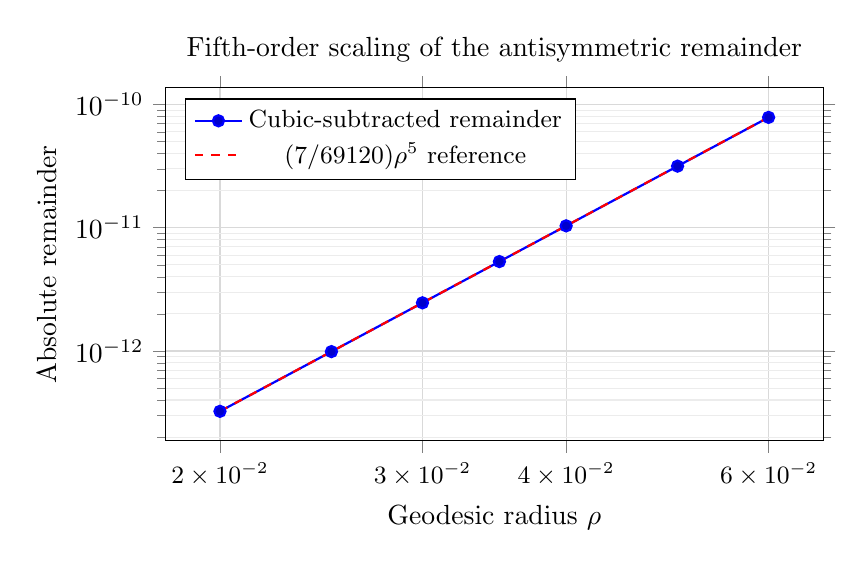
\begin{tikzpicture}
\begin{axis}[
  width=0.82\textwidth,
  height=0.50\textwidth,
  xmode=log,
  ymode=log,
  xtick={0.02,0.03,0.04,0.06},
  xticklabels={
    {$2\times10^{-2}$},
    {$3\times10^{-2}$},
    {$4\times10^{-2}$},
    {$6\times10^{-2}$}
  },
  xticklabel style={font=\small},
  xlabel={Geodesic radius $\rho$},
  ylabel={Absolute remainder},
  title={Fifth-order scaling of the antisymmetric remainder},
  grid=both,
  minor grid style={draw=gray!15},
  major grid style={draw=gray!30},
  tick align=outside,
  legend style={
    font=\small,
    at={(0.03,0.97)},
    anchor=north west
  }
]

\addplot+[
  thick,
  mark=*,
  mark size=2pt
] coordinates {
  (0.020,3.240218268562314e-13)
  (0.025,9.887464735749895e-13)
  (0.030,2.460044969256419e-12)
  (0.035,5.316430203679303e-12)
  (0.040,1.036368563834094e-11)
  (0.050,3.161599392313317e-11)
  (0.060,7.863586799957866e-11)
};
\addlegendentry{Cubic-subtracted remainder}

\addplot+[
  thick,
  dashed,
  mark=none
] coordinates {
  (0.020,3.240740740740741e-13)
  (0.025,9.889955873842595e-13)
  (0.030,2.460937500000000e-12)
  (0.035,5.319055627893521e-12)
  (0.040,1.037037037037037e-11)
  (0.050,3.164785879629631e-11)
  (0.060,7.875000000000000e-11)
};
\addlegendentry{$(7/69120)\rho^5$ reference}

\end{axis}
\end{tikzpicture}
\caption{Fifth-order scaling of the antisymmetric remainder after subtraction
of the known cubic term.}
\label{fig:rho5scaling}
\end{figure}

\begin{figure}[htbp]
\centering
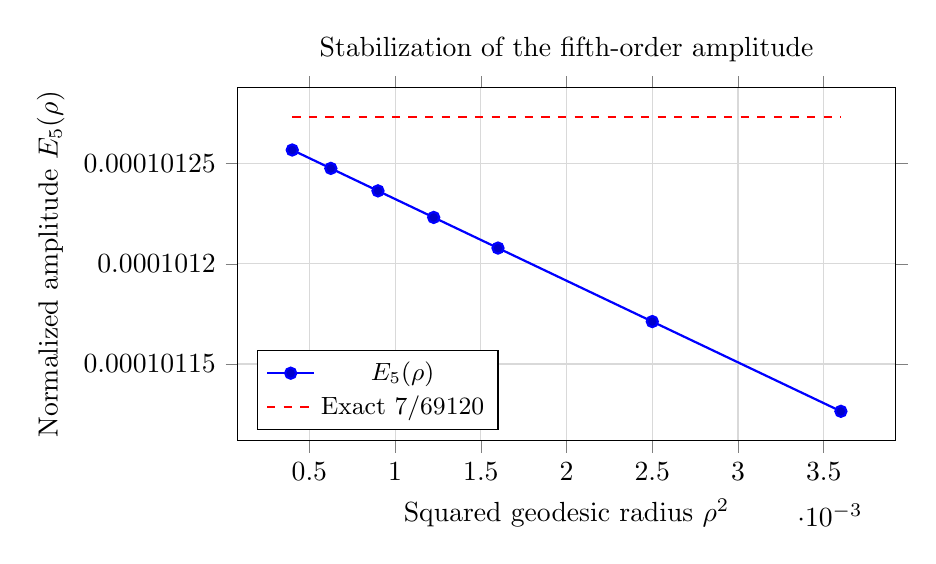
\begin{tikzpicture}
\begin{axis}[
  width=0.82\textwidth,
  height=0.50\textwidth,
  xlabel={Squared geodesic radius $\rho^2$},
  ylabel={Normalized amplitude $E_5(\rho)$},
  title={Stabilization of the fifth-order amplitude},
  grid=both,
  minor grid style={draw=gray!15},
  major grid style={draw=gray!30},
  tick align=outside,
  scaled y ticks=false,
  yticklabel style={
    /pgf/number format/fixed,
    /pgf/number format/precision=8
  },
  xticklabel style={
    /pgf/number format/fixed,
    /pgf/number format/precision=4
  },
  legend style={
    font=\small,
    at={(0.03,0.03)},
    anchor=south west
  }
]

\addplot+[
  thick,
  mark=*,
  mark size=2pt
] coordinates {
  (0.000400,0.0001012568208925723)
  (0.000625,0.0001012476388940789)
  (0.000900,0.0001012364184879185)
  (0.001225,0.0001012231608958991)
  (0.001600,0.0001012078675619232)
  (0.002500,0.0001011711805540261)
  (0.003600,0.0001011263734562483)
};
\addlegendentry{$E_5(\rho)$}

\addplot+[
  thick,
  dashed,
  mark=none
] coordinates {
  (0.000400,0.0001012731481481481)
  (0.003600,0.0001012731481481481)
};
\addlegendentry{Exact $7/69120$}

\end{axis}
\end{tikzpicture}
\caption{Stabilization of the normalized fifth-order amplitude toward the
exact target $7/69120$.}
\label{fig:rho5amplitude}
\end{figure}

The maximum nested-window spread in $C_3$ was approximately $2.58\times10^{-25}$, the largest turning-point shooting residual was below $9.84\times10^{-49}$, and independent precision/quadrature and angular-grid audits reproduced the extrapolated amplitude.  Thus the zero-curvature fifth-order combination is independently validated on this torus configuration.

\subsection{Overdetermined four-latitude fifth-order audit}
To test the $K\nabla_wK$ multiplier and to introduce a negative-curvature configuration, the same intrinsic-geodesic calculation was run at $\theta=\pi/4$, $\pi/3$, $\pi/2$, and $2\pi/3$, again with $w=e_\theta$ and its reverse.  Each run used 60-decimal arithmetic with 48-node Gauss--Legendre quadrature and an independent 70-decimal, 64-node precision/quadrature audit.  All polynomial least-squares fits were solved by high-precision QR factorization rather than normal equations.  A target-free odd fit
\[
A(\rho)=a_3\rho^3+a_5\rho^5+a_7\rho^7+a_9\rho^9
\]
was used to extract the fifth-order amplitude $a_5$ without fixing the cubic coefficient.

\begin{table}[htbp]
\centering
\caption{Independent fifth-order meridional amplitudes from four torus latitudes.  The numerical column is the unrestricted fitted $a_5$ from the 70-decimal audit.}
\label{tab:four-latitude-q5}
\begin{tabular}{rrrr}
\toprule
$\theta$ & $K$ & predicted $Q_5$ & unrestricted fitted $a_5$\\
\midrule
$\pi/4$ & $0.1907435698305462$ & $1.104442495077554\times10^{-4}$ & $1.104442495119574\times10^{-4}$\\
$\pi/3$ & $1/7$ & $1.157225393783871\times10^{-4}$ & $1.157225393876608\times10^{-4}$\\
$\pi/2$ & $0$ & $1.012731481481481\times10^{-4}$ & $1.012731481389811\times10^{-4}$\\
$2\pi/3$ & $-1/5$ & $2.626943724812797\times10^{-4}$ & $2.626943723695210\times10^{-4}$\\
\bottomrule
\end{tabular}
\end{table}
The relative errors in these four unrestricted fifth-order amplitudes are respectively $3.80\times10^{-11}$, $8.01\times10^{-11}$, $9.05\times10^{-11}$, and $4.25\times10^{-10}$.  These per-latitude comparisons are the direct numerical tests of the analytic coefficient.

For the same four latitudes, let the rows of the $4\times3$ matrix $M$ be
\[
\bigl(K\nabla_wK,\ \nabla_w\Delta K,\ \nabla^3K(w,w,w)\bigr).
\]
The matrix has rank three.  A high-precision QR least-squares solve of the overdetermined system $M\beta=a_5$ gives
\[
\beta=(-0.00820312499900897,\,-0.000607638888658034,\,0.00212673611057080),
\]
for the multipliers of $K\nabla_wK$, $\nabla_w\Delta K$, and $\nabla^3K(w,w,w)$, respectively.  The exact analytic values are
\[
\left(-\frac{21}{2560},-\frac7{11520},\frac{49}{23040}\right),
\]
and the corresponding relative differences are $1.21\times10^{-10}$, $3.80\times10^{-10}$, and $2.54\times10^{-10}$.  The residual norm is $2.18\times10^{-15}$, or $6.73\times10^{-12}$ relative to the norm of the measured amplitude vector; the numerical $2$-norm condition number of $M$ is approximately $86.76$.  Thus the fourth latitude supplies genuine redundancy: the recovered multipliers are consistent with all four independently fitted amplitudes rather than being forced by a square three-by-three solve.

\paragraph{Scope of the numerical tests.}
All torus runs use meridional directions $w=\pm e_\theta$ on a single ring torus ($R=3$, $r=1$). On this torus $\Hess K(w,w)=K''$ and $\Hess K(Jw,Jw)=(f'/f)K'$ vary independently along the meridian, so the quartic comparison does probe the two Hessian multipliers separately. No azimuthal run ($w=e_\phi$) has been performed at order $\rho^5$; such a run would give an additional test of the $Jw$-orientation structure. The invariant basis used in the four-latitude recovery is justified analytically (\cref{sec:symmetry}); the numerics confirm the multipliers within that basis.

\FloatBarrier
\section{Independent verification of the symbolic chain}\label{sec:verify}

This section records checks performed on October 25, 2026 in an AI-assisted review. They are independent re-implementations and consistency tests of the \emph{symbolic} chain; none of them rederives Brewin's formulas, and the original symbolic review did not rerun the torus geodesic computations of \cref{sec:numerics}; the subsequent independent $\theta=\pi/3$ run is distinguished in item (g). The single script \texttt{curvature\_v24\_checks.py} reproduces items (a), (b), (d), (e), and (g) below; item (f) refers to a separate script.

\begin{enumerate}[leftmargin=2em,label=(\alph*)]
\item \textbf{Side-law extraction.} Starting from the squared side law \eqref{eq:full-square} with $A_2,\dots,A_5$ as displayed, the coefficients $p_2,\dots,p_5$ and $r_2,\dots,r_5$ of \eqref{eq:p2r2}--\eqref{eq:p5r5}, the ratios \eqref{eq:ratio4} and \eqref{eq:ratio5ordered}, the invariant form \eqref{eq:ratio5}, and all nine multipliers of \eqref{eq:baker-main} were recomputed in exact arithmetic and agree.
\item \textbf{Surface contraction of Brewin's formulas.} The degree-six and degree-seven expressions of Appendix~\ref{app:source} were contracted on a surface in a second, independent implementation (and again in a third, written from Brewin's published equations with all third-derivative components $T_{abc}$ treated as independent). All three reproduce Propositions~\ref{prop:H6} and~\ref{prop:H7} identically, including the cancellation of $H_{12}$ and of the coefficients of $K_J,T_{001},T_{010},T_{100},T_{111}$.
\item \textbf{Comparison with Brewin's printed text (externally reported).} An independent reviewer reports comparing Eqs.~11.21b--e of arXiv:0903.2087v3 (revised November 4, 2022) with \eqref{eq:brewin-b}, \eqref{eq:brewin-c}, and the expressions in Appendix~\ref{app:source}: 1, 2, 7, and 17 terms respectively, 27 in all. Coefficients, index placement, derivative-slot order, and block structure reportedly agree, including the previously uninspected tail of Eq.~11.21e. The reviewer reports seven intentional single-term corruptions were all detected. This comparison concerns Brewin's \emph{printed arXiv text}, not an independent derivation or comparison with his Cadabra source. The comparison program \texttt{brewin\_1121\_transcription\_check.py} was described by the reviewer but was not supplied for local execution or inclusion in the present archive. Accordingly, this source-comparison result is recorded as externally reported, not locally reproduced. (The sign-convention lock $\BRiem=-\Riem$ is checked separately in \cref{sec:verify}.)
\item \textbf{Endpoint-swap symmetry.} Let $P=\exp_pX$ and $Q=\exp_pY$. Interchanging $P$ and $Q$ replaces $(X,D)$ by $(X+D,-D)$, preserves homogeneous degree, and leaves $d^2$ unchanged; hence every homogeneous term satisfies $H_n(X,D)=H_n(X+D,-D)$. After surface reduction (using the relations of Lemma~\ref{lem:commutator}), both $H_6$ and $H_7$ as transcribed in Appendix~\ref{app:source} satisfy this identity for generic $X,D$. The test has power: changing any single coefficient of $H_7$ by one unit destroys the symmetry, with the exception of the $+10$ term of the first block, which agrees with Brewin's printed text according to the comparison reported in item~(c). The symmetry thus independently constrains the same coefficients that item~(c) compares with the printed text. The test is insensitive to the sign convention of the commutator in Lemma~\ref{lem:commutator}; that sign is instead fixed by item~(e) and by the four-latitude fits. The symmetry is a necessary consistency condition on the source formulas, not a derivation of them.
\item \textbf{Ordered third derivatives.} The relations \eqref{eq:T-relations}, in particular $T_{101}-T_{011}=K\nabla_wK$, $T_{110}=T_{101}$ and $\nabla_w\Delta K=T_{000}+T_{011}$, were verified directly from the metric of the ring torus at general $\theta$, together with the exact anchors $Q_3=-7/1536$, $Q_5=7/69120$ and the five quartic anchors of \cref{tab:q4anchors}.
\item \textbf{Coefficient chain (separate audit).} An independent script (\texttt{curvature\_coefficient\_chain\_audit.py}) takes the surface-reduced coefficients as inputs and verifies the quotient $b_3/b_1$ through $\rho^5$, the general-$q$ factor, the $q=4/3$ specialization, and the constant-curvature check; it agrees with item~(a). The companion closeout archive now includes this script and its checksum.
\item \textbf{Tabulated numerics (from reported values).} The predicted quartic and quintic amplitudes at the four latitudes, the quoted relative differences, the residual-law ratios, and the $4\times3$ least-squares recovery of the weight-five multipliers (including the residual norm $2.18\times10^{-15}$ and the condition number $86.76$) were recomputed from the fitted amplitudes \emph{as reported} in \cref{sec:numerics} and agree. The underlying four-latitude fits were not regenerated in this original audit. A subsequent independent run regenerated the $\theta=\pi/3$ meridional fit at 60-digit working precision using 48-node quadrature, returning an unrestricted fifth-order amplitude $a_5=1.157225393876608\times10^{-4}$ to the displayed digits. The remaining three latitude fits have not been independently rerun in that subsequent check.
\end{enumerate}

\begin{table}[htbp]
\centering
\caption{Summary of the independent verification layers and what each does and does not establish.}
\begin{tabular}{lll}
\toprule
layer & establishes & does not establish\\
\midrule
(a), (f) extraction & algebra from $A_m$ to \eqref{eq:baker-main} & values of $A_4,A_5$\\
(b) contractions & surface reduction of Appendix A & that Appendix A matches Brewin (see (c))\\
(c) text comparison & printed 11.21b--e: 27 terms (reported) & correctness of Brewin; Cadabra comparison\\
(d) swap symmetry & coefficients consistent with $d^2$ symmetric & derivation of Brewin's formula\\
(e) torus identities & commutator lemma, anchors & --\\
(g) numerical checks & reported tables; $\pi/3$ fit rerun & other three fits rerun\\
\bottomrule
\end{tabular}
\end{table}

\FloatBarrier
\section{Reproducibility, scope, and limitations}\label{sec:repro}

The verification record identifies the following scripts (items 6--9 were added in version~2.4). The companion closeout archive includes the recovered scripts and numerical packages identified in its checksum manifest; scripts absent from that archive are historical references and are not asserted to be reproduced by this release:
\begin{enumerate}[leftmargin=2em]
\item \texttt{verify\_brewin\_degree6\_surface\_reduction.py}, which performs the generic lower-order convention lock, encodes Brewin 11.21d, reduces the degree-six tensors, and checks all quartic coefficients and torus anchors;
\item \texttt{verify\_brewin\_degree7\_surface\_reduction.py}, which repeats the convention lock, encodes Brewin 11.21e, reduces the degree-seven tensors, verifies orientation cancellation, and derives the fifth-order invariant coefficient;
\item \texttt{audit\_ordered\_derivatives\_torus.py}, which constructs the torus Christoffel symbols, Hessian, and ordered third derivatives from the metric and checks the commutator identities for general $\theta$;
\item \texttt{rho5\_torus\_high\_precision\_validation.py}, which performs the original zero-curvature high-precision geodesic calculation;
\item \texttt{rho5\_torus\_multilatitude\_validation.py}, which generalizes the intrinsic-geodesic calculation to an arbitrary meridional base latitude and is used here at $\theta=\pi/4$, $\pi/3$, $\pi/2$, and $2\pi/3$; it also extracts $Q_4$ from symmetric averages and uses QR-based polynomial least squares;
\item \texttt{curvature\_independent\_audit.py}, an independent contraction audit written from Brewin's published Eqs.~11.21d--e, with arbitrary independent third-derivative components;
\item \texttt{curvature\_coefficient\_chain\_audit.py}, the independent coefficient-chain audit of \cref{sec:verify}(f);
\item \texttt{curvature\_v24\_checks.py}, which reproduces the checks of \cref{sec:verify} (a), (b), (d), (e), and (g); and
\item \texttt{brewin\_1121\_transcription\_check.py}, an externally reported term-by-term source-comparison checker (not supplied or executed in this archive).
\end{enumerate}
The supplied symbolic verification scripts use exact arithmetic. The separately archived numerical reproduction records side samples, fitted coefficients, diagnostics, environment metadata, and checksums.
The public project repository is \url{https://github.com/CWBaker360/curvature-deformed-arcsine}.  The companion closeout archive supplies SHA-256 checksums of its included files. Historical scripts not in that archive are not included in the accompanying evidence; no GitHub release tag is claimed.

The result is local in $\rho$ and in the error variable $e$.  No global
convergence or large-radius assertion is made.

\paragraph{Higher-dimensional outlook.}
The same encode--scale--decode construction can be formulated on a
higher-dimensional Riemannian manifold $(M,g)$ after choosing an oriented
orthonormal two-frame $(w,v)$ in $T_pM$.  This two-frame determines the
oriented tangent plane
\[
\Pi=\Span\{w,v\},
\]
which contains the symmetric endpoint rays.  At leading curvature order,
one naturally expects the Gaussian curvature appearing in the surface
formula to be replaced by the sectional curvature $K_p(\Pi)$ of this plane.

At higher orders, however, the coefficients need not reduce to scalar
combinations of a single curvature function.  They may involve contractions
of the full Riemann tensor $\Riem$, its covariant derivatives
$\nabla^{(k)}\Riem$, the metric $g$, and the distinguished vectors $w$ and $v$.
Consequently, the resulting invariant basis may depend not only on the plane
$\Pi$, but also on the distinguished directions within that plane.

Unlike the surface case, a single unit vector $w\in T_pM$ does not determine
a canonical rotation operator on the full tangent space $T_pM$.  Once an
oriented two-plane $\Pi$ has been chosen, there is a canonical quarter-turn
\[
J_{\Pi}\colon \Pi\longrightarrow\Pi,
\qquad
J_{\Pi}w=v,
\qquad
J_{\Pi}v=-w,
\]
but this operator has no canonical extension to all of $T_pM$.  An auxiliary
choice of $v\perp w$, or equivalently of an oriented orthonormal two-frame,
is therefore required to define the symmetric endpoint geometry.

A higher-dimensional classification would consequently require both a
larger invariant basis and a precise account of the resulting two-frame
dependence.  Establishing such a classification is a natural extension of
the present work, but lies outside its scope.  The surface result obtained
here provides a foundational model for understanding how local geometric
invariants are organized within the Baker cubic refinement coefficient.

The normal-coordinate expansion and natural-tensor organization are
classical.  The result establishes the explicit coefficients for this
particular intrinsic refinement law and does not claim a new general theory
of local invariants.

\section{Conclusion}

The cubic coefficient of the intrinsic encode--scale--decode law separates successive layers of local geometry.  The universal Euclidean coefficient is followed by Gaussian curvature, its directional derivative, an even weight-four combination of quadratic curvature and Hessian data, and an odd weight-five combination of $K\nabla_wK$, $\nabla_w\Delta K$, and $\nabla^3K(w,w,w)$.  The coefficients are derived analytically from source-locked normal-coordinate formulas, verified by exact symbolic computation, and checked against classical and constant-curvature geometry.  Independent high-precision intrinsic-geodesic computations recover the quartic coefficient from symmetric averages and, across four torus latitudes including $K<0$, give an overdetermined fifth-order test that numerically recovers all three weight-five invariant multipliers.

For the Baker scale $q=4/3$, the complete result through fifth order is \eqref{eq:baker-main}.  This gives an explicit curvature extension of the Euclidean cubic refinement law, derived from Brewin's published two-point distance expansion and checked as described in \cref{sec:verify,sec:numerics}, and explicitly identifies the successive local curvature invariants encoded by its cubic coefficient.  The derivation is conditional on those source formulas, whose transcription has been compared with the published text (\cref{sec:verify}(c)) but not rederived.

\section*{AI-assistance and provenance disclosure}
AI tools were used in reviewing this manuscript and in the independent verification of \cref{sec:verify}: re-implementing the surface contractions, re-deriving the side-law extraction, testing the endpoint-swap symmetry, and recomputing tabulated quantities from reported values. The original torus geodesic computations of \cref{sec:numerics} are author-side results; a subsequent independent review regenerated the single $\theta=\pi/3$ fit, but not the complete four-latitude dataset. The author retains responsibility for the stated mathematical claims.

\section*{Acknowledgment}
The author acknowledges Rouben Rostamian's public documentation and analysis of the original approximate-trisection construction, and Leo Brewin's public release of the corrected normal-coordinate paper and its Cadabra source repository.

\begin{thebibliography}{99}

\bibitem{Bertrand1848}
J.~Bertrand,
\emph{D\'emonstration d'un th\'eor\`eme de M. Gauss},
Journal de Math\'ematiques Pures et Appliqu\'ees, 1st series, \textbf{13} (1848), 80--82.

\bibitem{Brewin2009}
L.~Brewin,
\emph{Riemann normal coordinate expansions using Cadabra},
Classical and Quantum Gravity \textbf{26} (2009), 175017;
arXiv:0903.2087v3, revised November 4, 2022.
\url{https://doi.org/10.1088/0264-9381/26/17/175017}

\bibitem{BrewinRepository}
L.~Brewin,
\emph{riemann-normal-coords: LaTeX and Cadabra sources for Riemann normal coordinate expansions},
GitHub repository, accessed August 5, 2026.
\url{https://github.com/leo-brewin/riemann-normal-coords}

\bibitem{Diguet1848}
C.-F.~Diguet,
\emph{Note de M. Diguet},
Journal de Math\'ematiques Pures et Appliqu\'ees, 1st series, \textbf{13} (1848), 83--86.

\bibitem{Gilkey}
P.~B. Gilkey,
\emph{Invariance Theory, the Heat Equation, and the Atiyah--Singer Index Theorem},
2nd ed., CRC Press, Boca Raton, 1995.

\bibitem{GrahamKuo2026}
C.~R. Graham and T.-M. Kuo,
\emph{Geodesic normal coordinates and natural tensors for pseudo-Riemannian submanifolds},
Proceedings of the American Mathematical Society \textbf{154} (2026), no.~1, 339--351.
\url{https://doi.org/10.1090/proc/17432}


\bibitem{Gray1974}
A.~Gray,
\emph{The volume of a small geodesic ball of a Riemannian manifold},
Michigan Mathematical Journal \textbf{20} (1973/74), 329--344.
\url{https://doi.org/10.1307/mmj/1029001150}

\bibitem{Pennec2019}
X.~Pennec,
\emph{Curvature effects on the empirical mean in Riemannian and affine manifolds: a non-asymptotic high concentration expansion in the small-sample regime},
arXiv:1906.07418, 2019.
\url{https://arxiv.org/abs/1906.07418}

\bibitem{Puiseux1848}
V.~Puiseux,
\emph{Sur le m\^eme th\'eor\`eme},
Journal de Math\'ematiques Pures et Appliqu\'ees, 1st series, \textbf{13} (1848), 87--90.

\bibitem{Rostamian}
R.~Rostamian,
\emph{An angle trisection}, online geometry note documenting the approximate construction due to Wayne Baker, May 31, 2010; accessed August 5, 2026.
\url{https://userpages.umbc.edu/~rostamia/Geometry/trisect-baker.html}

\end{thebibliography}

\appendix

\section{Source formulas used for the higher-order distance terms}\label{app:source}
For transparency, this appendix records the two higher-order Brewin inputs in the notation $x=X$, $Dx=D=Y-X$, using the source array $\BRiem$ defined in \eqref{eq:brewin-array}.  These formulas are not rederived here; their role is as source data for the exact surface reductions, and their transcription is independently audited in the accompanying archive.

The degree-six term is
\begin{align*}
360H_6={}&X^aX^bD^cD^dD^eD^f
\left(-8g^{gh}\BRiem_{acdg}\BRiem_{befh}-6\nabla_{cd}\BRiem_{aebf}\right)\\
&+X^aX^bX^cD^dD^eD^f
\left(16g^{gh}\BRiem_{adbg}\BRiem_{cefh}-9\nabla_{da}\BRiem_{becf}-9\nabla_{ad}\BRiem_{becf}\right)\\
&+X^aX^bX^cX^dD^eD^f
\left(16g^{gh}\BRiem_{aebg}\BRiem_{cfdh}-18\nabla_{ab}\BRiem_{cedf}\right).
\end{align*}

The degree-seven term is
\begin{align*}
1080H_7={}&X^aX^bX^cD^dD^eD^fD^g
\bigl(-4g^{hi}\BRiem_{adeh}\nabla_f\BRiem_{bgci}
-24g^{hi}\BRiem_{adeh}\nabla_b\BRiem_{cfgi}\\
&\qquad+10g^{hi}\BRiem_{adeh}\nabla_i\BRiem_{bfcg}
+16g^{hi}\BRiem_{adbh}\nabla_e\BRiem_{cfgi}
-4\nabla_{dea}\BRiem_{bfcg}\\
&\qquad-4\nabla_{dae}\BRiem_{bfcg}-4\nabla_{ade}\BRiem_{bfcg}\bigr)\\
&+X^aX^bD^cD^dD^eD^fD^g
\bigl(-18g^{hi}\BRiem_{acdh}\nabla_e\BRiem_{bfgi}-3\nabla_{cde}\BRiem_{afbg}\bigr)\\
&+X^aX^bX^cX^dD^eD^fD^g
\bigl(24g^{hi}\BRiem_{aefh}\nabla_b\BRiem_{cgdi}
+24g^{hi}\BRiem_{aebh}\nabla_f\BRiem_{cgdi}\\
&\qquad+24g^{hi}\BRiem_{aebh}\nabla_c\BRiem_{dfgi}
-6\nabla_{eab}\BRiem_{cfdg}-6\nabla_{aeb}\BRiem_{cfdg}-6\nabla_{abe}\BRiem_{cfdg}\bigr)\\
&+X^aX^bX^cX^dX^eD^fD^g
\bigl(48g^{hi}\BRiem_{afbh}\nabla_c\BRiem_{dgei}-12\nabla_{abc}\BRiem_{dfeg}\bigr).
\end{align*}

\section{Reproducibility commands}\label{app:commands}
From the package root, the exact symbolic checks may be run with
\begin{verbatim}
python scripts/verify_brewin_degree6_surface_reduction.py
python scripts/verify_brewin_degree7_surface_reduction.py
python scripts/audit_ordered_derivatives_torus.py
\end{verbatim}
The high-precision numerical validation may be reproduced with
\begin{verbatim}
python scripts/rho5_torus_high_precision_validation.py \
  --output-dir outputs/recomputed --precision-audit
\end{verbatim}
The nonzero-curvature fifth-order audits may be reproduced with
\begin{verbatim}
python scripts/rho5_torus_multilatitude_validation.py --u0 pi/4 \
  --output-dir outputs/pi4 --precision-audit
python scripts/rho5_torus_multilatitude_validation.py --u0 pi/3 \
  --output-dir outputs/pi3 --precision-audit
python scripts/rho5_torus_multilatitude_validation.py --u0 2pi/3 \
  --output-dir outputs/2pi3 --precision-audit
\end{verbatim}
The numerical runs are substantially more expensive than the exact symbolic checks.

\section{Revision history}\label{app:history}
\textbf{Version 2.3 (September 29, 2026):} complete directional curvature expansion through $\rho^5$; Brewin-based derivation; torus validations; four-latitude fifth-order audit.

\textbf{Version 2.4 (October 25, 2026):} (1) wording of the rigor claim: the theorem is stated and described as proved relative to Brewin's published formulas (Theorem remark, abstract, Conclusion); (2) new Section~\ref{sec:verify} recording independent verification layers and their limits, with companion script \texttt{curvature\_v24\_checks.py}; (3) externally reported term-by-term comparison of Brewin's printed Eqs.~11.21b--e (27 terms) with Appendix A, including the previously uninspected tail of 11.21e; (4) endpoint-swap symmetry of $H_6,H_7$ as a consistency test; (5) clarification of the uniformity of the $\bigO(\rho^6)$ remainder and of the parity argument via the squared side law; (6) explicit statement of the scope of the numerical tests (meridional directions on one torus); (7) archive scripts extended and a provenance flag added; (8) AI-assistance disclosure and this history. No equation, coefficient, or numerical value of v2.3 was changed.



\noindent\textbf{October 29, 2026, version 2.5:} Added Lemma~\ref{lem:uniform-remainder} replacing the standing regularity assumption by a smooth Hadamard-factorization argument; recorded the independent $\theta=\pi/3$ fit reproduction. No coefficient in the main theorem was altered.
\end{document}